\documentclass[11pt,letterpaper,english]{article}
\usepackage[utf8]{inputenc}
\usepackage{tikz}
\usetikzlibrary{arrows}
\usetikzlibrary{calc}
\usepackage{amsfonts,amssymb,amsmath, amsthm}
\usepackage{color}
\usepackage{pgfplots}
\usepackage{pgfgantt}
\usepackage[colorlinks,urlcolor=black,citecolor=black,linkcolor=black,menucolor=black]{hyperref}

\begin{document}

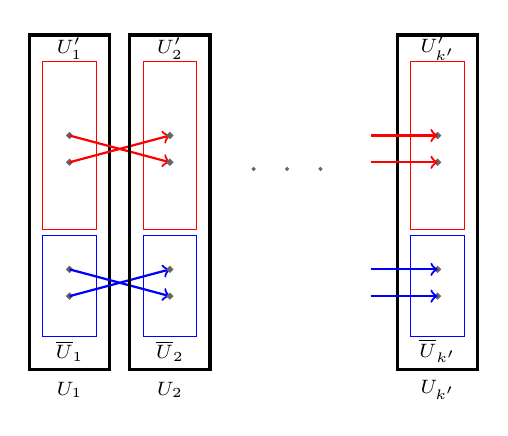
\begin{tikzpicture}
[scale=0.85,
 agent/.style={circle, draw=green!60, fill=green!5, very thick},
 good/.style={circle, draw=red!60, fill=red!5, very thick, minimum size=1pt},
]


\draw[black, very thick] (-0.6,-0.5-1) rectangle (0.6,3.5);

\draw[red] (-0.5+0.1,0.6) rectangle (0.5-0.1,3.1);
\node at (0, 3.3) {$\scriptstyle{U'_1}$};

\filldraw[color=black!60, fill=black!5, very thick](0, 2) circle (0.02);
\filldraw[color=black!60, fill=black!5, very thick](0, 1.6) circle (0.02);


\draw[blue] (-0.5+0.1,-1) rectangle (0.5-0.1,0.5);
\node at (0, -1.22) {$\scriptstyle{\overline{U}_1}$};

\filldraw[color=black!60, fill=black!5, very thick](0, 0) circle (0.02);
\filldraw[color=black!60, fill=black!5, very thick](0, -0.4) circle (0.02);

\draw[red, thick, ->]  (0,2)--(1.5, 1.6);
\draw[red, thick, ->]  (0,1.6)--(1.5, 2);

\draw[blue, thick, ->]  (0,0)--(1.5, -0.4);
\draw[blue, thick, ->]  (0,-0.4)--(1.5, 0);

\node at (0, -0.5-1.30) {$\scriptstyle{U_1}$};

\draw[black, very thick] (-0.6+1.5,-0.5-1) rectangle (0.6+1.5,3.5);

\draw[red] (1+0.1,0.6) rectangle (2-0.1,3.1);
\node at (0+1.5, 3.3) {$\scriptstyle{U'_2}$};


\filldraw[color=black!60, fill=black!5, very thick](1.5, 2) circle (0.02);
\filldraw[color=black!60, fill=black!5, very thick](1.5, 1.6) circle (0.02);

\draw[blue] (1+0.1,-1) rectangle (2-0.1,0.5);
\node at (1.5, -1.22) {$\scriptstyle{\overline{U}_2}$};

\filldraw[color=black!60, fill=black!5, very thick](1.5, 0) circle (0.02);
\filldraw[color=black!60, fill=black!5, very thick](1.5, -0.4) circle (0.02);

\node at (1.5, -0.5-1.30) {$\scriptstyle{U_2}$};

\draw[black, very thick] (-0.6+5.5,-0.5-1) rectangle (0.6+5.5,3.5);

\draw[red] (5+0.1,0.6) rectangle (6-0.1,3.1);
\node at (4+1.5, 3.3) {$\scriptstyle{U'_{k'}}$};


\filldraw[color=black!60, fill=black!5, very thick](5.5, 2) circle (0.02);
\filldraw[color=black!60, fill=black!5, very thick](5.5, 1.6) circle (0.02);

\draw[blue] (5+0.1,-1) rectangle (6-0.1,0.5);
\node at (5.5, -1.22) {$\scriptstyle{\overline{U}_{k'}}$};

\filldraw[color=black!60, fill=black!5, very thick](5.5, 0) circle (0.02);
\filldraw[color=black!60, fill=black!5, very thick](5.5, -0.4) circle (0.02);

\node at (5.5, -0.5-1.30) {$\scriptstyle{U_{k'}}$};

\draw[red, thick, ->]  (4.5,2)--(5.5, 2);
\draw[red, thick, ->]  (4.5,1.6)--(5.5, 1.6);

\draw[blue, thick, ->]  (4.5,0)--(5.5, 0);
\draw[blue, thick, ->]  (4.5,-0.4)--(5.5, -0.4);



\filldraw[color=black!60, fill=black, thick](2.75, 1.5) circle (0.01);
\filldraw[color=black!60, fill=black, thick](3.25, 1.5) circle (0.01);
\filldraw[color=black!60, fill=black, thick](3.75, 1.5) circle (0.01);
\end{tikzpicture}

\end{document}